\newpage
\section{C++}


\subsection{Why we need C++?}

\begin{question}{Why we need C++?}
	\begin{itemize}
		\item Fast program
		\item Take control of hardware.
	\end{itemize}
\end{question}


\subsection{How the C++ Compiler Works?}
\begin{question}{How the C++ Compiler Works?}
	It takes .cpp files and convert them into an intermediate format
	called an object file.

	Compilation stage:
	\begin{itemize}
		\item     1. preprocessing stage (output file extension :.i)
		\item     2. Compiling the source code. (output file extension :.s)
		\item     3. Assembling the compiled file. (output file extension :.o)
	\end{itemize}


	\begin{figure}[H]
		\centering
		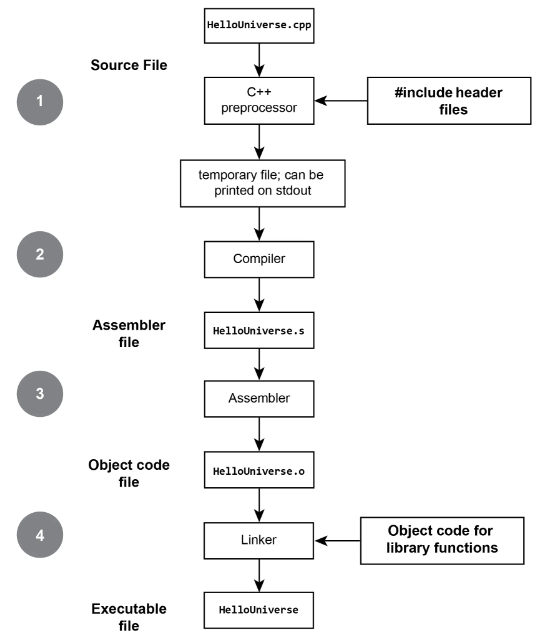
\includegraphics[width=0.5\textwidth]{p241.png}
		\caption{C++ compilation}
		\label{fig:p241}
	\end{figure}

\end{question}




\subsection{How the C++ Linker Works?}
The code shown in Lstlisting \ref{CPP:1} is \verb|mian.cc|, when we enter the command \verb|clang++  main.cc|, we got the error {\color{red}\verb|undefined reference to `log(char const*)'|}
Why do we get link error even if we don't use \verb|multiple| at all? This is becuase \verb|multiple| can be used in other files other than this file. 
We can make \verb|multiple| function only shown to this function by adding \verb|static| to its declaration.

% becuase multiple can be used in other files other than this file. We can make `multiple` function only shown to this function by adding `static` to its declaration.

\begin{lstlisting}[label={CPP:1},caption={main.cc}]
	#include <iostream>
	using namespace std;
	void log(const char* msg);
	int multiple(int a, int b){
		log("multiple");
		return a*b;
	}
	int main(){
	
	}
\end{lstlisting}




